% Tipos de datos geométricos: Euclidiano, Grafo, Variedad
% Compilar con: pdflatex tipos_datos_geometricos.tex
\documentclass[tikz,border=10pt]{standalone}
\usepackage{tikz}
\usetikzlibrary{calc, backgrounds}

\definecolor{gdlblue}{RGB}{41, 98, 168}
\definecolor{gdlred}{RGB}{191, 49, 49}
\definecolor{gdlgreen}{RGB}{30, 130, 76}
\definecolor{gdlorange}{RGB}{217, 130, 30}
\definecolor{gdlpurple}{RGB}{118, 56, 138}
\definecolor{gdlgray}{RGB}{140, 140, 140}
\definecolor{gdlyellow}{RGB}{190, 140, 10}

\begin{document}
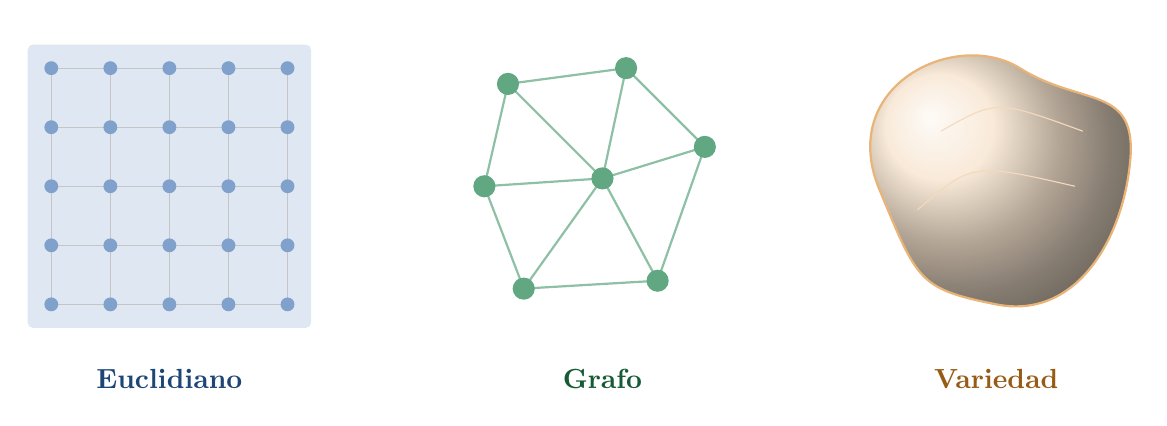
\begin{tikzpicture}

% === Panel izquierdo: Euclidiano (rejilla regular) ===
\begin{scope}[shift={(-5,0)}]
    % Fondo
    \begin{scope}[on background layer]
        \fill[gdlblue!15, rounded corners=2pt] (-0.3,-0.3) rectangle (3.3,3.3);
    \end{scope}

    % Aristas horizontales (4 aristas por fila, 5 filas)
    \foreach \x in {0,...,3} {
        \foreach \y in {0,...,4} {
            \draw[gdlgray!50] (\x*0.75, \y*0.75) -- (\x*0.75+0.75, \y*0.75);
        }
    }
    % Aristas verticales (5 columnas, 4 aristas por columna)
    \foreach \x in {0,...,4} {
        \foreach \y in {0,...,3} {
            \draw[gdlgray!50] (\x*0.75, \y*0.75) -- (\x*0.75, \y*0.75+0.75);
        }
    }

    % Nodos de la rejilla
    \foreach \x in {0,...,4} {
        \foreach \y in {0,...,4} {
            \fill[gdlblue!60] (\x*0.75, \y*0.75) circle (2.5pt);
        }
    }

    % Etiqueta
    \node[below, font=\bfseries, text=gdlblue!70!black] at (1.5, -0.7) {Euclidiano};
\end{scope}

% === Panel central: Grafo (topología irregular) ===
\begin{scope}[shift={(0.5,0)}]
    % Coordenadas de los nodos
    \coordinate (n1) at (0.3, 2.8);
    \coordinate (n2) at (1.8, 3.0);
    \coordinate (n3) at (0.0, 1.5);
    \coordinate (n4) at (1.5, 1.6);
    \coordinate (n5) at (2.8, 2.0);
    \coordinate (n6) at (0.5, 0.2);
    \coordinate (n7) at (2.2, 0.3);

    % Aristas
    \draw[gdlgreen!50, thick] (n1) -- (n2);
    \draw[gdlgreen!50, thick] (n1) -- (n3);
    \draw[gdlgreen!50, thick] (n1) -- (n4);
    \draw[gdlgreen!50, thick] (n2) -- (n4);
    \draw[gdlgreen!50, thick] (n2) -- (n5);
    \draw[gdlgreen!50, thick] (n3) -- (n4);
    \draw[gdlgreen!50, thick] (n3) -- (n6);
    \draw[gdlgreen!50, thick] (n4) -- (n5);
    \draw[gdlgreen!50, thick] (n4) -- (n6);
    \draw[gdlgreen!50, thick] (n4) -- (n7);
    \draw[gdlgreen!50, thick] (n5) -- (n7);
    \draw[gdlgreen!50, thick] (n6) -- (n7);

    % Nodos (dibujados encima de las aristas)
    \foreach \n in {n1,n2,n3,n4,n5,n6,n7} {
        \fill[gdlgreen!70] (\n) circle (4pt);
    }

    % Etiqueta
    \node[below, font=\bfseries, text=gdlgreen!70!black] at (1.5, -0.7) {Grafo};
\end{scope}

% === Panel derecho: Variedad (geometría continua) ===
\begin{scope}[shift={(5.5,0)}]
    % Superficie tipo blob orgánico con gradiente 3D
    \shade[ball color=gdlorange!25, opacity=0.9]
        (0.0, 1.5) .. controls (-0.5, 2.8) and (1.0, 3.5) .. (1.8, 3.0)
        .. controls (2.6, 2.5) and (3.3, 2.8) .. (3.2, 1.8)
        .. controls (3.1, 0.8) and (2.5, -0.2) .. (1.5, 0.0)
        .. controls (0.5, 0.2) and (0.5, 0.3) .. (0.0, 1.5);
    \draw[thick, gdlorange!60]
        (0.0, 1.5) .. controls (-0.5, 2.8) and (1.0, 3.5) .. (1.8, 3.0)
        .. controls (2.6, 2.5) and (3.3, 2.8) .. (3.2, 1.8)
        .. controls (3.1, 0.8) and (2.5, -0.2) .. (1.5, 0.0)
        .. controls (0.5, 0.2) and (0.5, 0.3) .. (0.0, 1.5);

    % Líneas de curvatura sutiles
    \draw[gdlorange!30, thin]
        (0.5, 1.2) .. controls (1.2, 1.8) .. (2.5, 1.5);
    \draw[gdlorange!30, thin]
        (0.8, 2.2) .. controls (1.5, 2.6) .. (2.6, 2.2);

    % Etiqueta
    \node[below, font=\bfseries, text=gdlorange!70!black] at (1.5, -0.7) {Variedad};
\end{scope}

\end{tikzpicture}
\end{document}
